% vim: set wrap


Most game playing programs build a game tree, and then chose the most promising move at the root of the tree.

\section{Minimax}

The minimax algorithm is the foundation of all game playing algorithms. The goal is the find the minimax value of a state or set of states, or equivalently of a set of moves, and then choose the move with the highest value. All values are from the perspective of the root player. The value of a node for the root player is the maximum of its children nodes, and the minimum for the opponent's children. The pseudocode for a simple depth first search version is shown in Figure \ref{fig:minimaxcode}.

\begin{figure}

\begin{lstlisting}
int minimax(State state){
	if(state.terminal())
		return state.value();
	int value;
	if(state.player() == WHITE){
		value = -INF;
		foreach(state.successors as succ)
			value = max(value, minimax(succ));
	}else{
		value = INF;
		foreach(state.successors as succ)
			value = min(value, minimax(succ));
	}
	return value;
}
\end{lstlisting}

\caption{Minimax Pseudocode}
\label{fig:minimaxcode}

\end{figure}


\subsection{Negamax}

Minimax uses values as taken from a fixed perspective of the root player. This complicates the code with having to minimize for one player and maximize for the other. Noting that $max(a,b) = -min(-a,-b)$, the duplication can be removed by negating the value each time we switch perspective. In this setup all values returned from an evaluation function are from the perspective of the player who is making the move. The pseudocode for this transformation is shown in Figure \ref{fig:negamaxcode}.

\begin{figure}

\begin{lstlisting}
int negamax(State state){
	if(state.terminal())
		return state.value();
	int value = -INF;
	foreach(state.successors as succ)
		value = max(value, -negamax(succ));
	return value;
}
\end{lstlisting}

\caption{Negamax Pseudocode}
\label{fig:negamaxcode}
\end{figure}

Several algorithms shown later reference the negamax formulation, and mean that the perspective shifts after every move.


\section{Alpha-Beta}\label{sec:alphabeta}

Alpha-beta ($\alpha\beta$) is a refinement of minimax, ignoring or pruning parts of the game tree that are provably unreachable if both players play perfectly. It maintains two values that bound the minimum value each player is guaranteed given the tree searched so far. When these bounds meet or cross, this is called a cut-off, and the remaining moves need not to be considered.

The pseudocode for alpha-beta, written in the negamax formulation, is shown in Figure \ref{fig:abcode}. It is a depth first implementation that returns after a maximum depth is reached. If a terminal node is found, the true value is returned, otherwise a heuristic value is returned.

\begin{figure}

\begin{lstlisting}
int alphabeta(State state, int depth, int alpha, int beta){
	if(state.terminal() || depth == 0)
		return state.value();
	foreach(state.successors as succ){
		alpha = max(alpha, -alphabeta(succ, depth-1, -beta, -alpha))
		if(alpha >= beta)
			break;
	}
	return alpha;
}
\end{lstlisting}

\caption{Alpha-beta Pseudocode, shown in the negamax formulation}
\label{fig:abcode}
\end{figure}

The runtime of alpha-beta is depends on the branching factor $b$, search depth $d$, and the number of cut-offs. Minimax has a runtime of $O(b^d)$, as does alpha-beta if it has no cut-offs. Given perfect move ordering, only the first move for the root player need be considered, leading to a runtime of $O(b^{d/2})$, an exponential speedup. In general, we don't have perfect move ordering, so the runtime will be between these two extremes.

\subsection{Transposition Table}

Transpositions can lead to an exponential blowup in the search space. To minimize the number of transpositions reevaluated, all strong alpha-beta based programs use a transposition table. Transpositions are usually found by comparing hash values and indexing into a large table. Sometimes a hash table is used, but usually the number of nodes searched is too big to store in memory, so a simple replacement policy is used. The simplest is to use the hash value as an index into a large array of values, replacing the previous node that indexed to the same location.

In many games this leads to a large speedup as the number of nodes searched is decreased dramatically.


\subsection{Iterative Deepening}

The runtime of alpha-beta is exponential in the search depth, and the strength of a player is dependent on a large search depth. If the algorithm is stopped before completion, the best move may not have been explored at all, so a shallower search that finishes is likely better than a deeper search that doesn't. Thus we start with a shallow search, and run a deeper search if we have time. This is not a big waste of work since the branching factor is at least two and so majority of the runtime is spent at the deepest level anyway. Iterative deepening allows alpha-beta to act as a breadth-first search with the memory overhead of a depth-first search.

Iterative deepening, when combined with a transposition table, also gives better move ordering. A node's value from the previous iteration gives a more accurate estimate of the value of a node than a heuristic estimate without a search. As we saw in Section \ref{sec:alphabeta}, better move ordering can lead to an exponential speedup, easily offsetting the overhead from searching the shallow depths multiple times.

\subsection{History Heuristic}

A good move ordering can lead to many cutoffs and an associated speed increase. The history heuristic is a game independent move ordering heuristic that gives higher priority to moves that have a track record of leading to cutoffs elsewhere in the tree. If a particular move gives a cutoff, it's quite likely that it will also give a cutoff for all of its siblings and so should have a higher priority there. This assumes that similar moves in different parts of the tree are related.




\section{Proof Number Search} \label{sec:PNS}

Proof Number Search (PNS) is a best-first search used to answer binary questions such as the outcome of a 2-player game starting from a given state. Being a binary outcome with the minimax property, it is well represented as an AND/OR tree when all values are from the perspective of the root player. Each node in the tree can have one of three values: Proven/Win, Disproven/Loss, or Unknown. All nodes store two numbers that show how close it is to being proven or disproven. The proof number (pn) is the minimum number of leaf nodes in the subtree that must be proven for the node to be proven. The disproof number (dn) is the minimum number of leaf nodes in the subtree that must be disproven for the node to be disproven. Some leaf nodes, if solved, will change the proof number of the root. Other leaf nodes, if solved, will change the disproof number of the root. Others, if solved, won't affect the proof or disproof numbers of the root. The Most Proving Nodes (MPN) are the intersection of the set that affect the proof number and the set that affect the disproof number at the root. Solving an MPN will definitely affect either the proof or disproof number of the root. Every tree is guaranteed to have at least one MPN. Proof Number search grows its tree by continually expanding an MPN. Proof Number search can be split into 3 phases: descent, expansion, and update.

The most proving node is found during the descent phase. It can be found by selecting the child with the minimum proof number when at an OR node and by selecting the child with the minimum disproof number when at an AND node, applying this iteratively until a leaf node is reached. This leaf node is an MPN.

Once the most proving node $n$ is found, it is expanded, initializing all non-terminal children with $n_i.pn = 1, n_i.dn = 1$, winning children with $n_i.pn = 0, n_i.dn = \infty$ and losing children with $n_i.pn = \infty, n_i.dn = 0 $, where $n_i$ refers to the $i^{th}$ child of $n$.

After expansion, the proof and disproof numbers of all the ancestors of the most proving node must be updated using these formulas. For OR nodes: $$ n.pn = \displaystyle\min\limits_{i=0}^k n_i.pn,\quad n.dn = \displaystyle\sum\limits_{i=0}^k n_i.dn $$ For AND nodes: $$ n.pn = \displaystyle\sum\limits_{i=0}^k n_i.pn, \quad n.dn = \displaystyle\min\limits_{i=0}^k n_i.dn $$ Note how this backs up a single win at an OR node as a win, or a single loss at an AND node as a loss. It also backs up all losses at an OR node as a loss, or all wins at an AND node as a win. % Everywhere else it represents the optimistic lower bound on the number of nodes that must be (dis)proven to (dis)prove the current node.

These three phases are repeated until the root is solved or the tree grows too big to be stored in memory. At the root, if $r.pn = 0$ it is solved as a win, or if $r.dn = 0$ it is solved as a loss, otherwise it is still unknown.

\begin{figure}
\centering
\ovalbox{
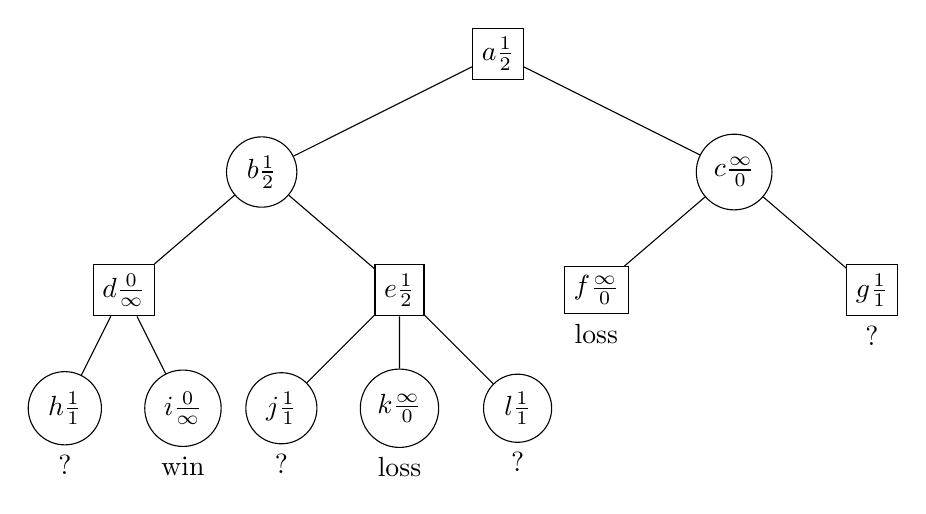
\begin{tikzpicture}[
	level distance=15mm,
	level 1/.style={sibling distance=60mm},
	level 2/.style={sibling distance=35mm},
	level 3/.style={sibling distance=15mm},
	]
\node [rectangle,draw] (z){$a \frac{1}{2}$}
  child {node [circle,draw] {$b \frac{1}{2}$}
    child {node [rectangle,draw] {$d \frac{0}{\infty}$}
      child {node [circle,draw,label=below:?] {$h \frac{1}{1}$}}
      child {node [circle,draw,label=below:win] {$i \frac{0}{\infty}$}}
    }
    child {node [rectangle,draw] {$e \frac{1}{2}$}
      child {node [circle,draw,label=below:?] {$j \frac{1}{1}$}}
      child {node [circle,draw,label=below:loss] {$k \frac{\infty}{0}$}}
      child {node [circle,draw,label=below:?] {$l \frac{1}{1}$}}
    }
  }
  child {node [circle,draw] {$c \frac{\infty}{0}$}
    child {node [rectangle,draw,label=below:loss] {$f \frac{\infty}{0}$}}
    child {node [rectangle,draw,label=below:?] {$g \frac{1}{1}$}}
  };
\end{tikzpicture}}
\caption{Proof Number search tree, Squares are OR nodes, Circles are AND nodes, proof numbers are on top, disproof numbers on the bottom, based on \cite{winands2003-PDS-PN}}
\label{fig:pntree}
\end{figure}

Consider the tree in Figure \ref{fig:pntree}. The most proving node is found by following the edges $a \rightarrow b \rightarrow e \rightarrow j$. If $j$ has a child that is a win, it would be backed up as a win at $j$, leading to a win at $e$, and a win at $b$, giving the root player a winning move from the root. With $a.pn = 1$ at the root, only 1 node was needed to be proven as a win for the root to also be proven as a win. If both $j$ and $l$ were proven to be losses, then $e$ would be a loss, leading $b$ to also be a loss, and consequently the root to also be a loss. This is reflected in $a.dn = 2$ at the root. If, however, $j$ has 1 non-terminal child $m$ and no terminal children, $m$ would have $m.pn = 1, m.dn = 1$ and would be the new MPN. If $j$ has 2 non-terminal children and no terminal children, $j.pn = 2, j.dn = 1$, and $l$ would be the new MPN.

This algorithm selects nodes based on the shape and value of the tree, using no domain or game specific heuristic. It is guided towards slim parts of the tree, areas where there are few moves available, or where many moves are forced. In many games it is advantageous to have more moves available, or higher mobility, than your opponent. Proof Number search is very fast at solving these positions. In games or positions where the branching factor is constant or consistent, with few forced moves, Proof Number search approximates a slow breadth-first search, and thus isn't very fast.

Being a best-first search algorithm, the whole tree must be kept in memory, since any node could become the MPN and therefore be searched at any time. This makes it a very memory intensive search algorithm, with many of the variants attempting to reduce memory usage, allowing bigger problems to be solved.

One simple optimization is to stop the update phase once the proof and disproof numbers don't change. This often happens when siblings have the same value, causing the sibling to be the new MPN. A new search can be started from this node instead of from the root. A simple memory optimization is to remove and reuse the memory of subtrees under a proven or disproven node.

\subsection{The Negamax Formulation} \label{sec:NegaPDS}

\begin{figure}
\centering
\ovalbox{
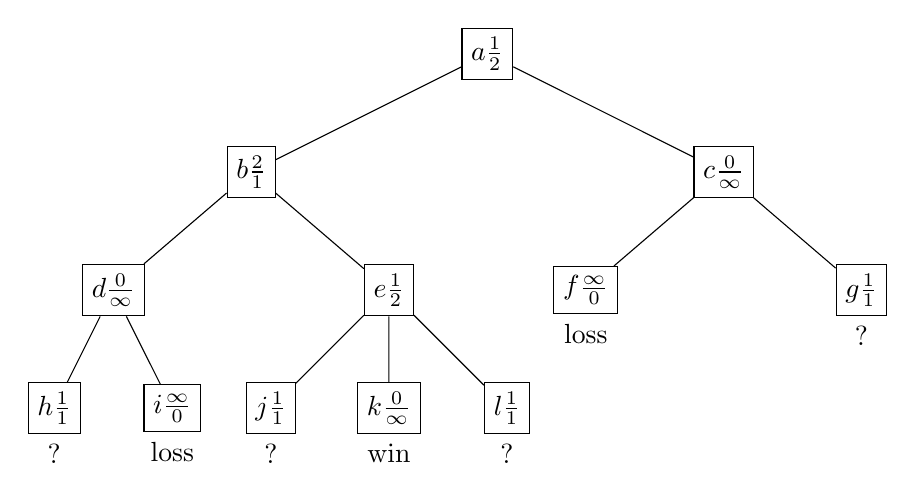
\begin{tikzpicture}[
	level distance=15mm,
	level 1/.style={sibling distance=60mm},
	level 2/.style={sibling distance=35mm},
	level 3/.style={sibling distance=15mm},
	]
\node [rectangle,draw] (z){$a \frac{1}{2}$}
  child {node [rectangle,draw] {$b \frac{2}{1}$}
    child {node [rectangle,draw] {$d \frac{0}{\infty}$}
      child {node [rectangle,draw,label=below:?] {$h \frac{1}{1}$}}
      child {node [rectangle,draw,label=below:loss] {$i \frac{\infty}{0}$}}
    }
    child {node [rectangle,draw] {$e \frac{1}{2}$}
      child {node [rectangle,draw,label=below:?] {$j \frac{1}{1}$}}
      child {node [rectangle,draw,label=below:win] {$k \frac{0}{\infty}$}}
      child {node [rectangle,draw,label=below:?] {$l \frac{1}{1}$}}
    }
  }
  child {node [rectangle,draw] {$c \frac{0}{\infty}$}
    child {node [rectangle,draw,label=below:loss] {$f \frac{\infty}{0}$}}
    child {node [rectangle,draw,label=below:?] {$g \frac{1}{1}$}}
  };
\end{tikzpicture}}
\caption{Proof Number search tree using the Negamax formulation, all nodes are OR nodes, $\phi$ is on top, $\delta$ is below, based on \cite{winands2003-PDS-PN}}
\label{fig:negamaxtree}
\end{figure}

Just like minimax can be written in the negamax formulation, so too can proof number search. The Proof number at an OR node is the same as the Disproof number at an AND node, and is named $\phi$ (phi). Similarly, the Proof number at an AND node is the same as the Disproof number at an OR node, and is named $\delta$ (delta). Instead of considering all nodes to be from the one player's perspective, all nodes are considered to be from the player who is making the move at that node. This shift in perspective greatly simplifies the code.

Figure \ref{fig:negamaxtree} shows the same tree as in Figure \ref{fig:pntree}, except using the negamax formulation. Note how all nodes are now OR nodes, and the proof and disproof numbers are exchanged in the nodes that were previously AND nodes.

Given this shift in perspective, the descent and update formulas need to be corrected. The new descent move selection is always to choose the child with the minimum delta. The new update formulas are: $$ n.\phi = \displaystyle\min\limits_{i=0}^k n_i.\delta, \quad n.\delta = \displaystyle\sum\limits_{i=0}^k n_i.\phi $$

\begin{figure}

\begin{lstlisting}
int pns(State state){
	Node root = initnode(state);
	while(root.phi != 0 && root.delta != 0) search(root, state);
	return (root.phi == 0 ? PROVEN : DISPROVEN);
}
void search(Node node, State state){
	if(node.numchildren == 0){ //found MPN
		foreach(state.successors as succ)
			node.addchild(initnode(succ));
	}else{
		do{
			Node child = node.child_min_delta();
			search(child, state.move(child.move));
			bool changed = updatePD(node);
		}while(!changed && node.phi != 0 && node.delta != 0);
	}
}
Node initnode(State state){
	Node node; node.move = state.lastmove();
	if(state.win()){       node.phi = 0;   node.delta = INF; }
	else if(state.loss()){ node.phi = INF; node.delta = 0;   }
	else{                  node.phi = 1;   node.delta = 1;   }
	return node;
}
bool updatePD(node){
	int phi = INF, delta = 0;
	foreach(node.children as child){
		phi = min(phi, child.delta);
		delta = delta + child.phi;
	}
	bool changed = (node.phi == phi && node.delta == delta);
	node.phi = phi; node.delta = delta;
	return changed;
}
\end{lstlisting}

\caption{Proof Number Search Pseudocode, shown in the negamax formulation, with the optimization to not propagate up if no changes occur}
\label{fig:pnscode}
\end{figure}

The pseudocode for Proof Number Search in the negamax formulation is shown in Figure \ref{fig:pnscode}.


\subsection{Transposition Table}

Proof number search uses an explicit tree which must be kept in memory, but the tree required is often bigger than available memory. One common approach to bounding the memory needed is to store the nodes in a transposition table instead of an explicit tree. This has the benefit of bounded memory as well as saving computation and memory on transpositions, at the cost of having to recompute nodes that are replaced in the transposition table. Even when a node needs to be recomputed, its children are often still in the transposition table, allowing for a quick recomputation. In many cases the transposition table can be several orders of magnitude smaller than would be needed to store the explicit tree.


\subsection{DF-PN: Depth First Proof Number search} \label{sec:DF-PN}

Depth First Proof Number search (DF-PN)\cite{nagai1999-DFPN} uses two thresholds which are set to express how long the MPN stays in the current subtree. The thresholds are calculated based on the realization that there is no need to update the parents $\phi$ and $\delta$ and do a new move selection if the next descent will go to the same child node. As long as the child's $\delta$ is smaller or equal to all of its siblings, an MPN still lies in its subtree. By staying within this subtree, fewer updates are needed, and locality is maintained, using fewer active nodes and needing less recomputation.

$n.th_\phi$ and $n.th_\delta$ are both set to $\infty$ at the root. $n.th_\phi$ and $n.th_\delta$ are computed as follows: $$n_c.th_\phi = n.th_\delta + n_c.\phi - \displaystyle\sum\limits_{i=0}^k n_i. \phi$$ $$n_c.th_\delta = min(n.th_\phi, n_2.\delta + 1)$$ where $n_c$ refers to the child with the smallest $\delta$ and $n_2$ is the child with the second smallest $\delta$. The search process continues at each node until $n.\phi \geq n.th_\phi$ or $n.\delta \geq n.th_\delta$.


\subsection{DF-PN+: DF-PN with Heuristics} \label{sec:DF-PN+}

So far proof number search assumes that all leaf nodes are equally hard to prove, using only proof and disproof numbers, or more generally, the shape of the tree. DF-PN+ adds two types of heuristic evaluation \cite{nagai-thesis}.

$h(n)$ is a heuristic evaluation of the expected difficulty of proving or disproving a node and its subtree. DF-PN has a constant $h(n) = 1$. A small value means that this node is expected to be easy to (dis)prove while a big value means this node is expected to be hard to (dis)prove. This value is used at node initialization of non-terminal nodes: $$n.\phi = h_\phi(n), \quad n.\delta = h_\delta(n), \quad h(n) \ge 1$$

$cost(n, n_c)$ is the cost for moving from a node to a child, and affects the shape of the tree. DF-PN has a constant $cost(n, n_c) = 0$. Small values encourage narrow and deep trees while large values encourage wide and shallow trees. This value is a penalty to going deeper, and could be used to encourage deeper trees on moves that are evaluated to be better, or to find shallower solutions.

Adding a non-zero $cost$ function means changing the update formulas:
$$ n.\phi = \displaystyle\min\limits_{i=0}^k (n_i.\delta + cost_\delta(n, n_c))$$ $$n.\delta = \displaystyle\sum\limits_{i=0}^k (n_i.\phi + cost_\phi(n, n_c))$$
as well as the threshold formulas:
$$n_c.th_\phi = n.th_\delta + n_c.\phi - \displaystyle\sum\limits_{i=0}^k (n_i.\phi - cost_\delta(n, n_i))$$ $$n_c.th_\delta = min(n.th_\phi, n_2.\delta + cost_\phi(n, n_2) + 1) - cost_\phi(n, n_c)$$

While the values initialized by $h$ are overwritten when its children are expanded, the $cost$ persists until the node is solved. Given fast and effective $h$ and $cost$ functions, DF-PN+ can solve problems significantly faster than DF-PN.

\subsection{The $1+\epsilon$ Trick} \label{sec:epstrick}

One weakness of Proof Number search in general is that it requires a large amount of memory to store the tree. Depth first variants and transposition tables help, but many problems we want to solve need trees that are several orders of magnitude bigger than available memory. In cases where the memory limit is particularly tight, DF-PN can spend a huge amount of time regenerating subtrees. To reduce this effect, the $1+\epsilon$ Trick \cite{pawlewicz2007epsilon} increases the thresholds exponentially instead of linearly.

Consider the case where two children of the root (so $\infty$ thresholds) are both promising, but also hard to solve. Since Proof Number search likes keeping all children at similar values, the two will get roughly equal time. Once the subtrees become big, the time spent on one will overwrite the nodes from the other tree. Once its $\delta$ exceeds the other, the search will switch, taking up a large amount of memory, and overwriting the nodes from the subtree of the first child. Since the threshold is one higher than the second smallest, they will swap every time the tree gets rebuilt to exceed the other child by one. This linear increase in the threshold can mean an exponential increase in time.

If the threshold was not simply the second smallest + 1, but instead a multiple of it, the investment into this subtree wouldn't be overwritten so easily by its equally challenging siblings. The $1 + \epsilon$ trick therefore is to replace the $n_c.th_\delta$ threshold from DF-PN with $$n_c.th_\delta = min(n.th_\phi, n_2.\delta*(1 + \epsilon))$$ where $\epsilon$ is some small positive value. This way $n_c.th_\delta$ increases by a constant multiple instead of a constant. It leads to $n_c$ being called at most $log_{1+\epsilon}n.th = O(\log n.th)$ times instead of linear times before reaching its parent's threshold.

This trick encourages DF-PN to be even more depth-first, causing lower memory usage, more efficient usage of the transposition table, and reducing the number of node recalculations. Note that it no longer follows the same order as the original PNS, sometimes expanding a node that isn't an MPN, and therefore it may do an unbounded amount of extra work.

$\epsilon = 0.25$ has been shown to work well in practice.


\section{Monte Carlo Tree Search}

For games where a very fast and effective evaluation function exists, alpha-beta search is likely to be fast and strong, but no good heuristic is known for many games including Go and Havannah. Monte Carlo Tree Search (MCTS) is an algorithm for building and exploring a game tree that is based on statistics instead of a heuristic evaluation function. MCTS avoids using a heuristic by building its tree as guided by playing random games. While a random move sequence by itself has a very low playing strength, in aggregate random games will favour the player that is in a better position.

MCTS consists of four phases which together are called a simulation. Each simulation adds some experience to the tree, updating the expected chance of winning for the nodes it traverses. These winning rates are stored as the number of wins and the number of simulations through a node. The notation is: $n.v$ for the winning rate and $n.n$ for number of simulations. The four phases are:
\begin{description}
\item[Descent] This phase descends the game tree from the root to a leaf node N in the game tree. At each node one of the available moves is selected according to some criteria based on the current winning rate and possibly heuristic knowledge. When the Upper Confidence Bounds (UCB) formula is used, this is called Upper Confidence Bounds applied to Trees (UCT), but other formulas such as RAVE have been developed and are commonly used.
\item[Expansion] If the node N has experience from a previous simulation, its children are expanded, increasing the size of the tree.
\item[Rollout] A random game is played from N through the newly expanded children, to the end of the game. Heuristics can be used to make the moves less random and more representative of a real game. The strength of the overall algorithm is highly dependent on the average outcome of the random games being representative of the strength of the position.
\item[Back-propagation] The outcome of the random game in the rollout is back propagated to the moves chosen in the tree. The winning rate of the moves made by the player that won the rollout is increased while winning rate of the moves by the player that lost the rollout is decreased.
\end{description}

...diagram needed...

These four steps are repeated continually until a stopping condition is reached, such as running out of time or memory. At this point a move is chosen by some criteria. The three most common criteria are: most simulations, most wins, and highest lower confidence bound on winning rate. The most simulations is the most conservative, but if a counter-move was found late in the game, it may still be the most simulated even if it doesn't have the highest winning rate. The most wins is a little less conservative and will favour a late new-comer if it has almost caught up. The highest winning rate is quite risky since it may favour a move that has a very small subtree where a good counter move exists but hasn't been found yet. To deal with that a lower bound can be used, but a large confidence interval should be used to avoid choosing risky moves.

The pseudocode for MCTS is shown in Figure \ref{fig:mctscode}.

\begin{figure}

\begin{lstlisting}
Move mcts(State state){
	Node root = Node(state);
	while(!timeout)
		search(root, state);
	return root.bestchild();
}
int search(Node node, State state){
	//rollout
	if(node.numchildren == 0 && node.sims == 0){
		while(!state.terminal())
			state.randmove();
		return (state.win() ? WIN : LOSS);
	}

	//expand
	if(node.numchildren == 0)
		foreach(state.successors as succ)
			node.addchild(Node(succ));

	//descent
	Node best;
	foreach(node.children as child)
		if(best.value() < child.value())
			best = child;

	int outcome = 1 - search(best, state.move(best.move));

	//back-propagate
	best.sims += 1;
	best.wins += outcome;
	return outcome;
}
\end{lstlisting}

\caption{Monte Carlo Tree Search, shown in the negamax formulation}
\label{fig:mctscode}
\end{figure}


Many extensions have been developed to increase the playing strength of MCTS. Some of these are explained below.

\subsection{UCT: Upper Confidence bounds as applied to Trees}\label{sec:uct}

The most common and most famous formula in MCTS is UCT. It derives from Upper Confidence Bounds (UCB), which is famously used on the multi-armed bandit problem. It is used to balance exploitation and exploration when multiple options are available and each option returns a random distribution of reward. The amount of regret, ie the number of plays to non-optimal arms, should be minimized to maximize reward in the long term.

The UCT formula is:
\begin{equation}\label{eqn:uct} n_i.v + c*\sqrt{\frac{\ln(n.n)}{n_i.n}}\end{equation}
where $c$ is a tunable constant to balance the exploration rate. This formula is used in the descent phase of MCTS to chose which move to make. Intuitively, moves with high winning rate should be exploited more, but moves with a small number of simulations as compared to the parent should be explored to improve the confidence. This formula is guaranteed to converge to a best move given infinite time and memory.




\subsection{RAVE: Rapid Action Value Estimate}\label{sec:rave}

In basic MCTS many thousands of simulations are run per second, but the information about which moves were made during the rollouts is unused. A win or a loss is composed of many moves which contribute to that outcome, and often good moves during a rollout are also good moves if made earlier during the rollout or descent phases. This is a similar to the reasoning behind the history heuristic. Thus, we can keep a winning rate for each move during the rollouts and use this to encourage exploration of moves that do well during rollouts. This information is gathered more quickly than by pure experience alone, though it is less correlated to success, and so should be phased out as real experience is gained. The notation used is $n.r$ for the RAVE winning rate and $n.m$ for the number of RAVE updates for a node.

Usually Rapid Action Value Estimate (RAVE) experience and real experience are combined as a linear combination, starting as only RAVE experience and asymptotically approaching only real experience, and replaces $n_i.v$ in Equation \ref{eqn:uct}:
\begin{equation}\label{eqn:rave1} \beta*n_i.v + (1-\beta)*n_i.r \end{equation}
Several formulas for $\beta$ have been proposed. The simplest two formulas for $\beta$ are:
\begin{equation}\label{eqn:rave2} \beta = \frac{k}{k+n_i.n} \end{equation}
\begin{equation}\label{eqn:rave3} \beta = \sqrt{\frac{k}{k+3*n_i.n}} \end{equation}
 both of which have a tunable constant $k$ which represents the midpoint, so how many simulations are needed for the RAVE experience and real experience to have equal weight.

David Silver computed an optimal formula for $\beta$ under the assumption of independence of estimates:
\begin{equation}\label{eqn:rave4} \beta = \frac{n_i.r}{n_i.n+n_i.r+4*n_i.n*n_i.r*b^2} \end{equation}
where $b$ is a tunable RAVE bias value.

In practice, RAVE leads to a large increase in playing strength for games such as Go and Havannah where the assumption that a good move is also good if played earlier. The RAVE updates often lead to sufficiently large exploration that the constant in the UCT exploration term is set very low or even to 0, removing UCT exploration altogether.

\subsection{Heuristic Knowledge}\label{sec:heuristicknowledge}

While UCT is guaranteed to converge given infinite time, game specific knowledge can encourage it to find good moves faster. When a node is expanded, its children all start with no experience, so the default policy is to choose between them randomly. The simulation is more representative of a good game, and leads to a better understanding of the minimax value, if it chooses a good move first. Eventually the best move will receive the majority of the simulations, and we'll do better if this is true right from the beginning. Each game has its own heuristics, and Havannah-specific ones are described in later chapters, but the way these heuristics is used is game independent.

The first way heuristic knowledge is used is to simply add fake experience to a node. Instead of initializing a node as $n_i.v = 0, n_i.n = 0$, good moves can be initialized with $n_i.v = a, n_i.v = b$, where $a$ and $b$ are tunable constants, which effectively means that this node has some amount of wins attributed to it before any simulations have gone through it. This has the effect of allowing the node to look good for the first while even if it is unlucky, but the extra simulations will fade over time as the few extra wins becomes insignificant in the long run. Bad moves can similarly be initialized with fewer wins than simulations effectively depressing its early winning rate. Depending on the implementation, this may encourage the first few simulations to avoid the good moves, due to their smaller confidence bounds compared to similar moves with the same high winning rate, which has the effect of making the grandparent move look bad. This knowledge could also be added as fake RAVE experience as well as, or instead of, actual experience.

Another way heuristic knowledge is used is to add a knowledge term to the value formula. This leaves the the experience and confidence bounds alone, but gives a boost for the first few simulations to nodes with higher knowledge. This has the added benefit of being able to order the nodes by boost size. The knowledge term should fall off with increasing experience. Three suggested knowledge terms are: $$\frac{n_i.k}{log(n_i.n)}, \quad \frac{n_i.k}{\sqrt{n_i.n}}, \quad \frac{n_i.k}{n_i.n}$$ where $n_i.k$ is the knowledge value for the node $n_i$.


\subsection{Rollout Policy}

As mentioned above, the strength of MCTS is highly dependent on the average outcome of the rollouts being representative of the strength of the position. When a player who is in a good position has an easy defence to a devastating attack, but fails to defend, the outcome is not representative of the strength of the original position. Decreasing randomness by enforcing defences against devastating attacks can bias the outcome, but usually leads to higher quality and more representative games, leading to a stronger player. Most rollout policies used in real programs are game specific, but a few game independent ones are mentioned here.

Instead of pure random, a weighted random scheme can be used. Moves that have good experience in the tree can be selected with a higher probability to poor moves. This could be based on real experience, RAVE experience, pattern knowledge or heuristic knowledge as described in the Section \ref{sec:heuristicknowledge}.

The Last Good Reply scheme can be used, where the moves made by the player that won a rollout are saved for use in later rollouts when similar situations occur. When these moves fail to lead to a win in a later rollout, they may be removed from the list of replies.

All possible moves can be checked to see if they lead to an instant win, in which case that move should be made. Similarly if this turn is skipped would each move lead to an instant loss if not made, in which case the defensive should be forced.



%\subsection{Other extensions}

%should any of these be described?

%\begin{itemize}
%\item parallelization
%\item dynamic widening
%\item Solution backups
%\item multiple rollouts per simulation
%\item avoid symmetries or transpositions
%\item first player urgency
%\end{itemize}

